\chapter{Results} \label{results}
%\begin{figure}[H]
%\centering
%    \begin{minipage}{0.45\textwidth}
%%        \centering
%        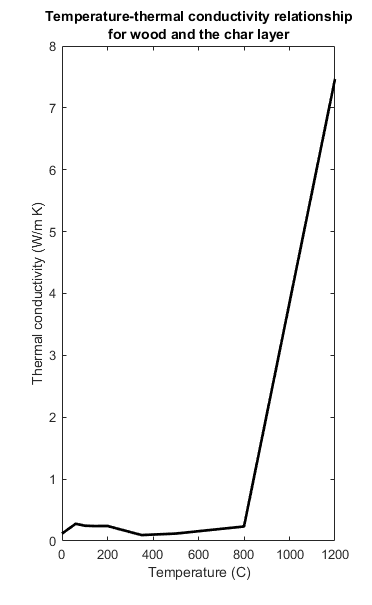
\includegraphics[width=0.9\textwidth]{figures/resultsk_cropped.png} % first figure itself
%        \caption{The resulting $\kappa$-values }
%        \label{kresult_fig}
%    \end{minipage}
%    \begin{minipage}{0.45\textwidth}
%%        \centering
%        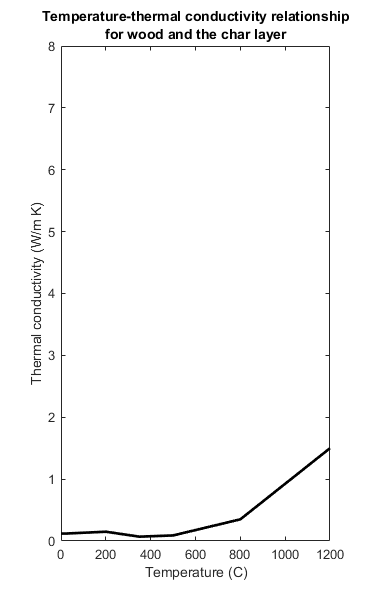
\includegraphics[width=0.9\textwidth]{figures/eurok_samescale_cropped.png} % second figure itself
%        \caption{The original $\kappa$-values}
%        \label{scalekeuro_fig}
%    \end{minipage}
%\end{figure}\

The results of the MCMC analysis as well as the MAP optimization is visualised in the section below.
\section{Resulting k-values}

The thermal conductivity ($\kappa$-values) at key temperatures integral to this project, the resulting values are shown in Table \ref{krestab}. 
As can be seen in Figure \ref{kresult_euro_fig} there was quite a drastic difference in the thermal diffusivity at 1200 \textdegree C and between 0\textdegree C and 200\textdegree C.
The large difference at 1200\textdegree C is due to how the model is created, at that temperature the majority of the heat is transferred through thermal radiation.
The model did not model thermal radiation separately but instead incorporated the radiation into a equivalent conduction.
Between 0\textdegree C and 200\textdegree C the modelling of the evaporation was moderately successful as a spike can be seen at 100 \textdegree C.  
\begin{figure}
\centering
	\label{kresult_euro_fig}
	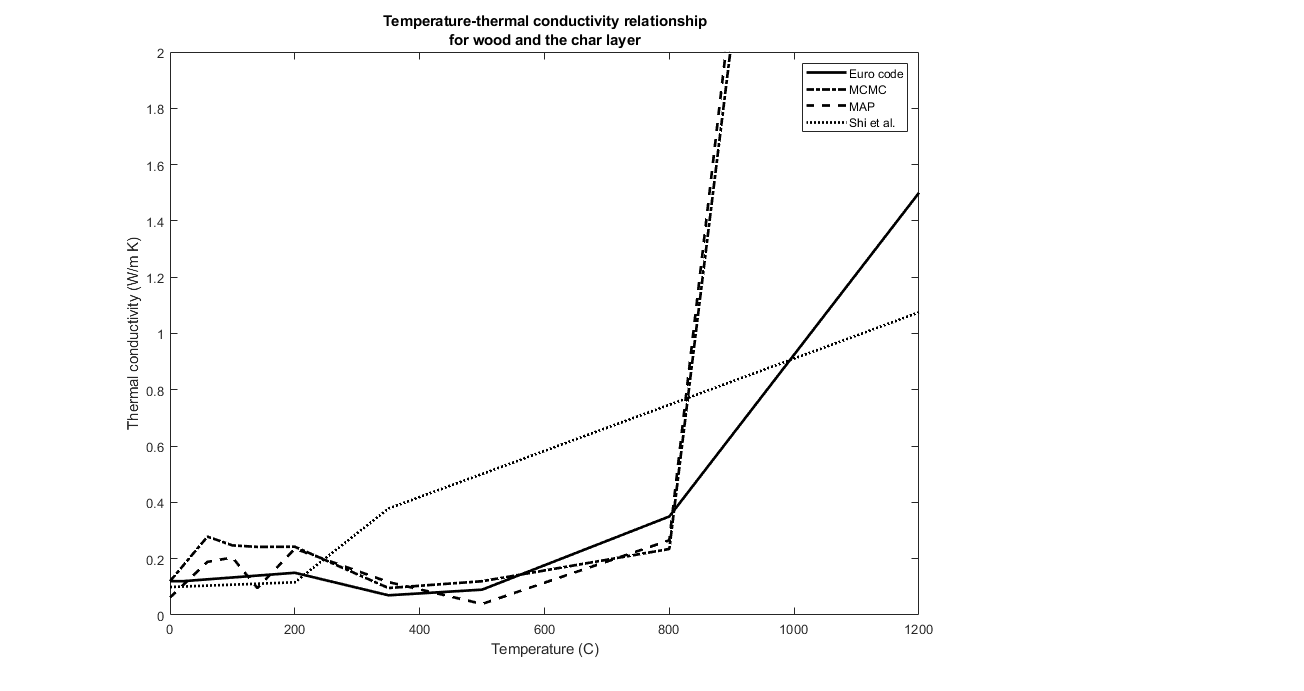
\includegraphics[width=\textwidth]{figures/kvalues_all_shi.png}
	\caption{Resulting $\kappa$ values compared to Euro-code standard values}
\end{figure}
\begin{table} \label{krestab}
\centering
	\begin{tabular}{ r r r r }
	\toprule
	 \textdegree C & EURO & MAP & MCMC\\
	\midrule
	0   & 0.12&0.062 &0.12\\
	60  &0.12& 0.189 &0.278\\
	100 &0.12& 0.204 &0.247\\
 	140 &0.12& 0.096 &0.242\\
	200 & 0.15& 0.2355 &0.243\\
	350 & 0.07& 0.117  &0.096\\
	500 & 0.09& 0.039 &0.120\\
	800 & 0.35& 0.265 &0.234\\
	1200& 1.5& 7.943 &7.467\\
	\bottomrule	
	\end{tabular}
	\caption{Resulting thermal conductivity in W/m$\cdot$K}
\end{table}
 
 For each temperature there will be a different distribution of samples. 
 In Figure \ref{histofig} The distribution of all the samples were plotted in a histogram with a kernel density estimation overlay. 
 The resulting $\kappa$-values from the MCMC algorithm is plotted in red and the Maximum a posteriori is plotted in blue.
 From the blue lines it is clear that the Nelder-Mead optimization was not run a sufficient amount of times as many of the values are not at the maximum but on the way to the maximum.
 At 140\textdegree C it can also be seen that the algorithm got stuck at a local maximum.
 
\begin{figure}[b]
\label{histofig}
\centering
	\begin{subfigure}{}
	\centering
	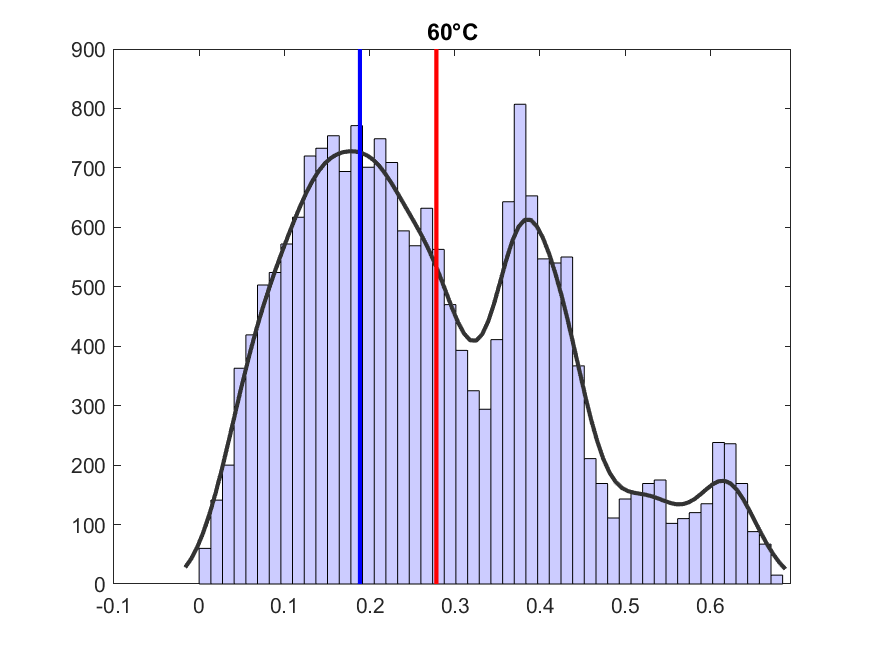
\includegraphics[width = 0.45\linewidth]{figures/histograph/histo1.png}
	\end{subfigure}
	\begin{subfigure}{}
	\centering
	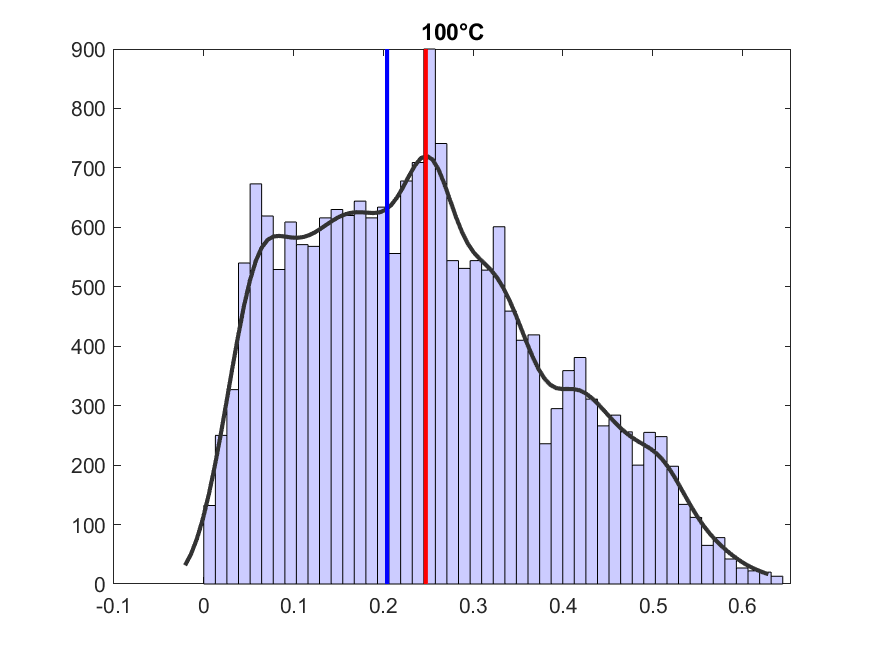
\includegraphics[width = 0.45\linewidth]{figures/histograph/histo2.png}
	\end{subfigure}
	\begin{subfigure}{}
	\centering
	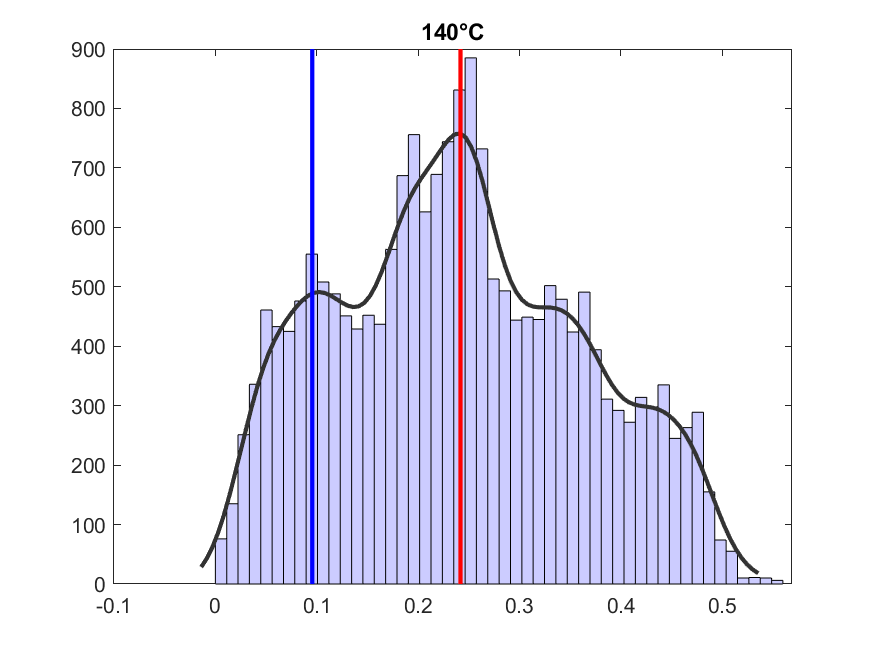
\includegraphics[width = 0.45\linewidth]{figures/histograph/histo3.png}
	\end{subfigure}
	\begin{subfigure}{}
	\centering
	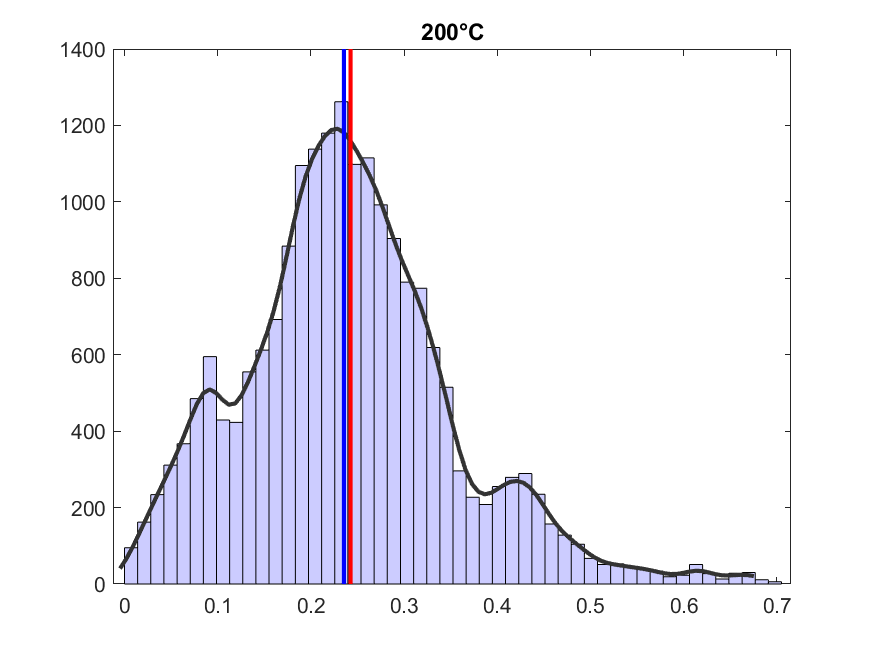
\includegraphics[width = 0.45\linewidth]{figures/histograph/histo4.png}
	\end{subfigure}
	\begin{subfigure}{}
	\centering
	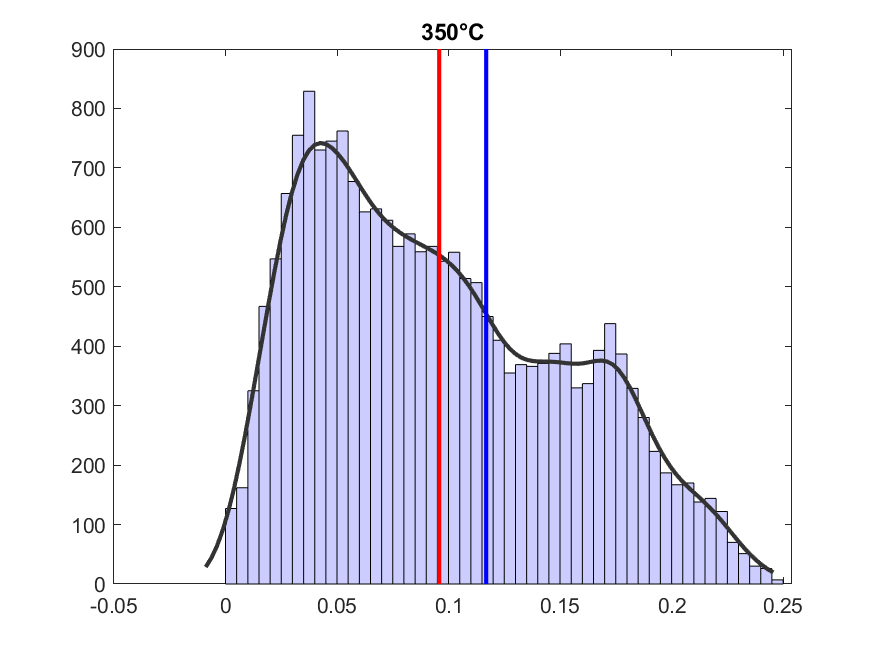
\includegraphics[width = 0.45\linewidth]{figures/histograph/histo5.png}
	\end{subfigure}
	\begin{subfigure}{}
	\centering
	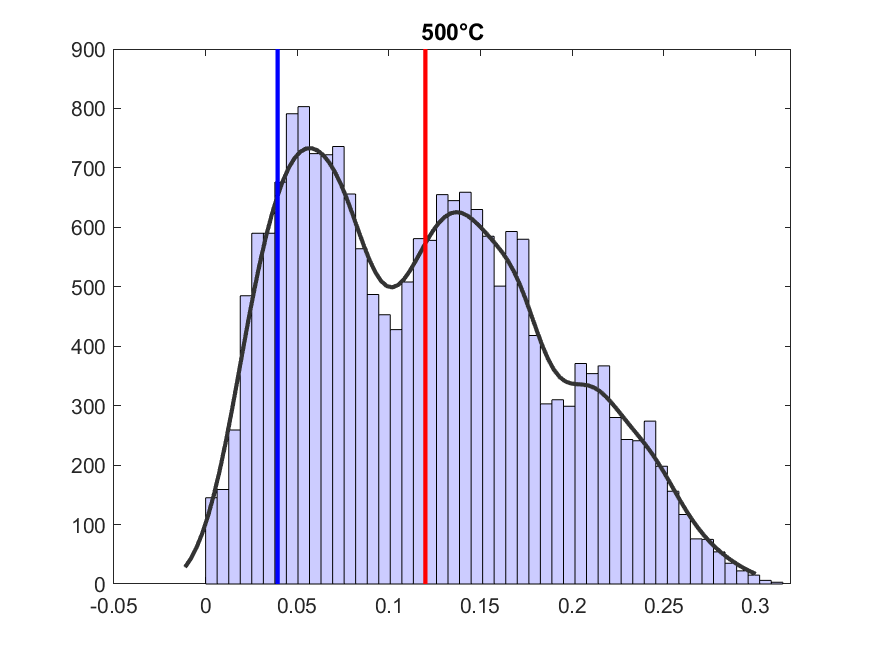
\includegraphics[width = 0.45\linewidth]{figures/histograph/histo6.png}
	\end{subfigure}
	\begin{subfigure}{}
	\centering
	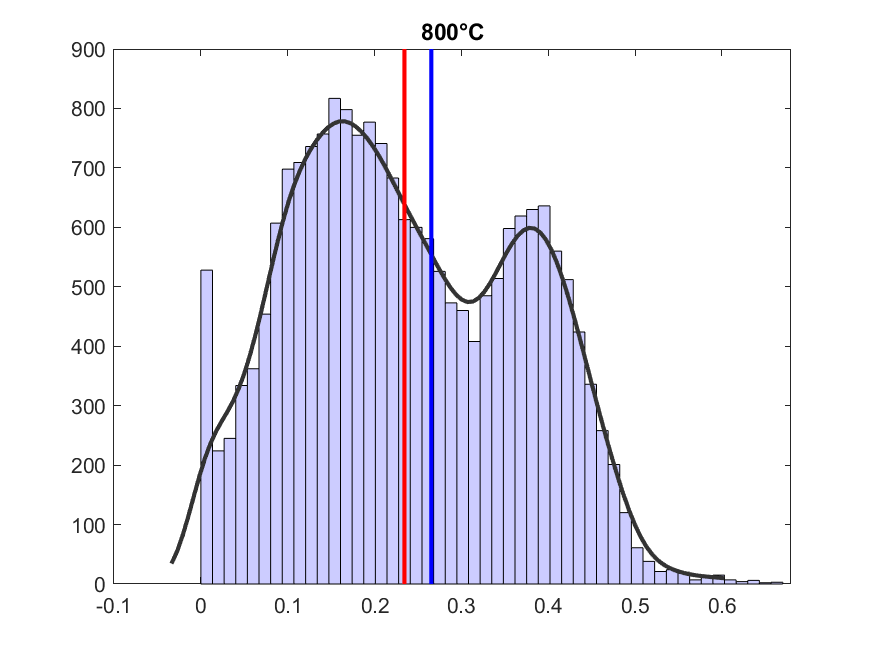
\includegraphics[width = 0.45\linewidth]{figures/histograph/histo7.png}
	\end{subfigure}
	\begin{subfigure}{}
	\centering
	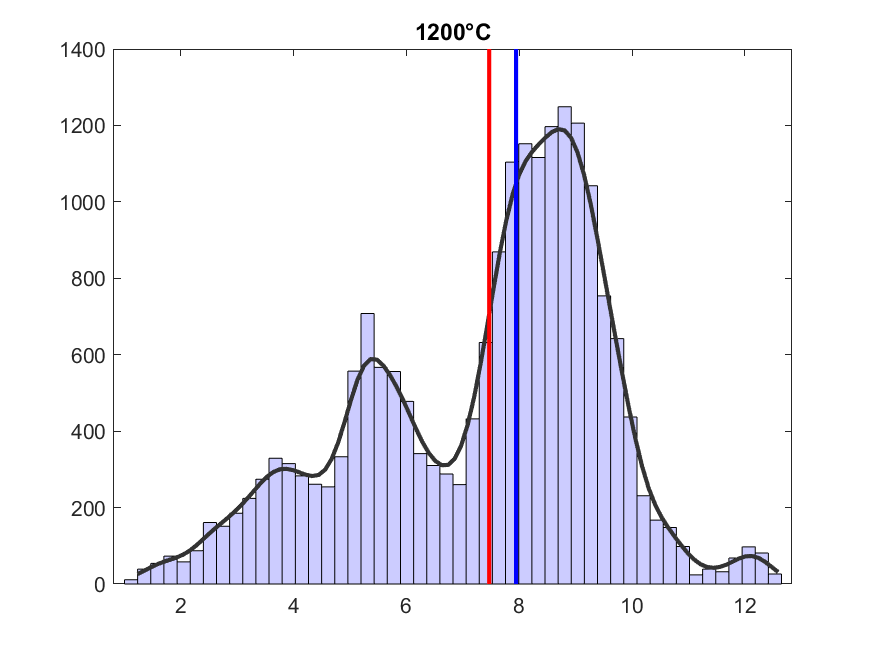
\includegraphics[width = 0.45\linewidth]{figures/histograph/histo8.png}
	\end{subfigure}
	\centering
	\begin{subfigure}{}
	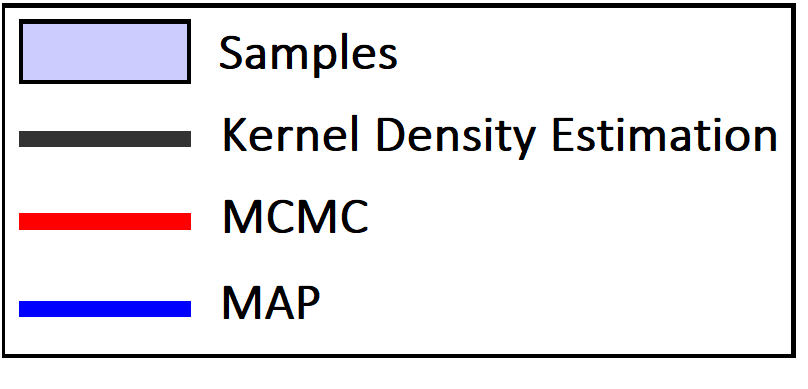
\includegraphics[width = 0.3\linewidth]{figures/histograph/legend.png}
	\end{subfigure}
	\caption[short]{Distribution of samples at different temperatures with MCMC and MAP results indicated}
\end{figure}

\subsection{Evaluation of error}
Despite the uncertainties connected to the problem, a quantifiable measure of error is still required to allow unbiased assessment of the success of the algorithm and results.
The obtained $\kappa$-values will be used to rerun the model and obtain the new modelled temperature for each depth. 
For each depth the error will be quantified using the norm of the relative error at the seven different depths, noted as $i$.
The relative error will be calculated according to  Equation \ref{relerror}. 
The new modelled output errors are compared to the EURO-code $\kappa$-value output errors to assess if the methods used produced a more accurate representation of the data.
The error at different depths are summarised in Table \ref{errortab} and the lowest error at that depth is highlighted in green. 
At a depth of 0mm none of the errors are highlighted as this temperature is independent of the $\kappa$-values.
This error measurement can be used to asses the error in the model or assumptions made to obtain the model.
It is important to note that this error does not only quantify the error in the thermal conductivity but any errors due to model assumptions are also encompassed.

\begin{equation}\label{relerror}
\epsilon(i) = \frac{\norm{\hat{x}(i)-x(i) }_2}{\norm{x(i)}_2} \quad \quad i= 1, ... ,7
\end{equation}

\begin{table}[H] \label{errortab}
\centering
	\begin{tabular}{ r r r r }
	\toprule
	Depth(mm) & Eurok & MAP & MCMC\\
	\midrule
	0 & 0.2886 & 0.2886 & 0.2886\\
	16.5 & 0.2166 & \cellcolor{green!20}0.1943 & 0.2050\\
	33 & 0.3008   & \cellcolor{green!20} 0.1905 & 0.2001\\
	49.5 & 0.5693 & 0.3482 &\cellcolor{green!20} 0.3227\\
	66 & 0.5467   & 0.3186 & \cellcolor{green!20}0.2673\\
	82.5 & 0.5012 &\cellcolor{green!20} 0.3394 & 0.3583\\
	99 & 0.2192   & 0.2190 &\cellcolor{green!20} 0.2185\\
	\bottomrule	
	\end{tabular}
	\caption{Summary of error between models and data}
\end{table}

\subsection{Thermal diffusivity}
The main intent of this project was to determine the thermal diffusivity of SA-Pine. 
In Table \ref{diffrestab} the resulting thermal diffusivity is shown.
The thermal diffusivity was calculated using the information in Table \ref{cptab} and Equation \ref{alphaeq}.

\begin{table}[H] \label{diffrestab}
\centering
	\begin{tabular}{ r r r r }
	\toprule
	Temp \textdegree C & Eurok & MAP & MCMC\\
	\midrule
	0&   $1.64\ten{-4}$&	$8.46\ten{-5}$&	$1.64\ten{-4}$\\
	60&  $1.64\ten{-4}$&	$2.58\ten{-4}$&	$3.79\ten{-4}$\\
	100& $1.64\ten{-4}$&	$2.78\ten{-4}$&	$3.37\ten{-4}$\\\
	140& $1.64\ten{-4}$&	$1.31\ten{-4}$&	$3.30\ten{-4}$\\
	200& $2.05\ten{-4}$&	$3.21\ten{-4}$&	$3.32\ten{-4}$\\
	350& $9.55\ten{-5}$&	$1.60\ten{-4}$&	$1.31\ten{-4}$\\
	500& $1.23\ten{-4}$&	$5.32\ten{-5}$&	$1.64\ten{-4}$\\
	800& $4.78\ten{-4}$&	$3.62\ten{-4}$&	$3.19\ten{-4}$\\
	1200& $2.05\ten{-3}$&	$1.08\ten{-2}$&	$1.02\ten{-2}$\\
	\bottomrule	
	\end{tabular}
	\caption{Resulting thermal diffusivity($\alpha$)in m/s$^2$}
\end{table}






